\chapter{Anexos}

\section{Cuestionario de Evaluación}

\begin{enumerate}
    \item El control de ``nivel de disparo'' (trigger level) sirve para:
    \begin{itemize}
        \item[B.] Ajustar el punto de inicio del barrido.
    \end{itemize}

    \item El selector de ``Fuente de disparo'' tiene la función de:
    \begin{itemize}
        \item[C.] Permite seleccionar entre disparo: Interno – Externo – Línea.
    \end{itemize}

    \item Relación entre modos de presentación dual:
    \begin{itemize}
        \item[A.] Barrido alternado: Se emplea cuando la velocidad de barrido es elevada. En un barrido se muestra un
            canal, y en el siguiente el otro.
        \item[B.] Barrido troceado (Chop): Se emplea cuando la velocidad de barrido es baja. Dentro de cada ciclo de
            barrido se va alternado cada uno de los canales.
    \end{itemize}

    \item En el modo normal, la base de tiempos se dispara cuando:
    \begin{itemize}
        \item[B.] El nivel de disparo está contenido entre el máximo y el mínimo de la señal de entrada.
    \end{itemize}

    \item El procedimiento de ``calibrar la punta de pruebas'' se realiza:
    \begin{itemize}
        \item[B.] Con la punta en posición X10 y es para compensar la respuesta en frecuencia.
    \end{itemize}

    \item El ajuste para la calibración de la punta suele encontrarse:
    \begin{itemize}
        \item[B.] En la propia punta de pruebas, y se accede mediante un destornillador de plástico.
    \end{itemize}

    \item El modo ``ADD'' con ``INV'' se utiliza para:
    \begin{itemize}
        \item[B.] Funcionar como un instrumento de canal único y entrada diferencial.
    \end{itemize}

    \item Determinación de parámetros en oscilograma (Eje Y=\qty{2}{V/div}, T=\qty{1}{ms/div}, Sonda X10):
    \begin{enumerate}
        \item \textbf{Ciclo de trabajo (D):}
        Observando el oscilograma de la consigna, se tiene que el periodo ocupa $T = 8 \text{ div}$ y el ancho de pulso
        es $t_o \approx 2 \text{ div}$.
        \[ D = \frac{t_o}{T} = \frac{2 \text{ div}}{8 \text{ div}} = 0.25 \]
        \item \textbf{Valor eficaz de la tensión ($V_{ef}$):}
        La amplitud pico a pico es de $V_{pp} = 6 \text{ div}$. Considerando la atenuación de la sonda:
        \[ V_{pp} = 6 \text{ div} \times \qty{2}{V/div} \times 10 = \qty{100}{V} \]
        Como la señal no tiene componente de CC, se utiliza la fórmula para un tren de pulsos bipolar simétrico:
        \[ V_{ef} = V_{pp} \sqrt{D - D^2} = \qty{100}{V} \times \sqrt{0.25 - 0.25^2} = \qty{100}{V} V\times 0.433 = \qty{43.3}{V} \]
    \end{enumerate}
\end{enumerate}

\section{Formas de onda a mano alzada}
A continuación se presentan los espacios para las formas de onda solicitadas según los roles asignados:

    \begin{figure}[H]
        \centering
        \textbf{ECG (Gaston Grasso):} Senoidal, \qty{500}{Hz}, \qty{3}{Vpp}, offset: \qty{2}{V}.
        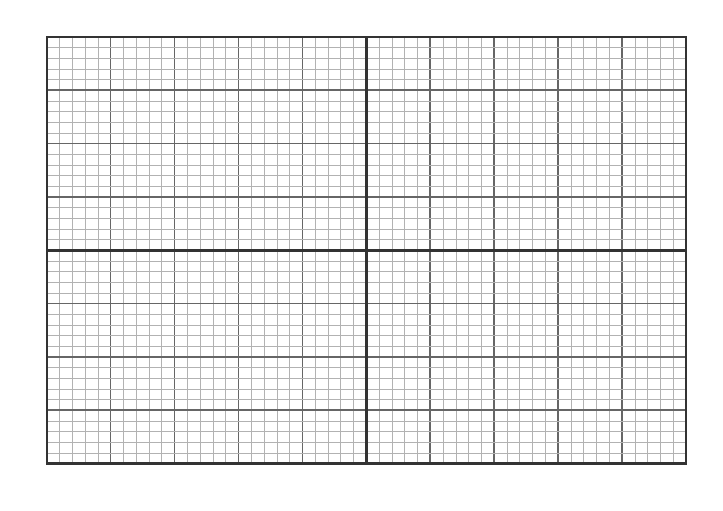
\begin{tikzpicture}
    \begin{axis}[
        width=0.8\textwidth,
        height=7cm,
        grid=both,
        major grid style={line width=.6pt,draw=black!60},
        minor grid style={line width=.2pt,draw=black!30},
        xmin=0, xmax=10,
        ymin=-4, ymax=4,
        xtick={0,1,2,3,4,5,6,7,8,9,10},
        ytick={-4,-3,-2,-1,0,1,2,3,4},
        minor x tick num=4,
        minor y tick num=4,
        xticklabels={},
        yticklabels={},
        tick style={draw=none},
        axis line style={draw=black!80, thick},
    ]
        % Ejes centrales más marcados
        \draw[line width=1pt, black!80] (axis cs:0,0) -- (axis cs:10,0);
        \draw[line width=1pt, black!80] (axis cs:5,-4) -- (axis cs:5,4);
    \end{axis}
\end{tikzpicture}

    \end{figure}

    \begin{figure}[H]
        \centering
        \textbf{EO1 (Angelo Prieto):} Senoidal, \qty{2550}{Hz}, \qty{8}{Vp}, offset: \qty{0}{V}.
        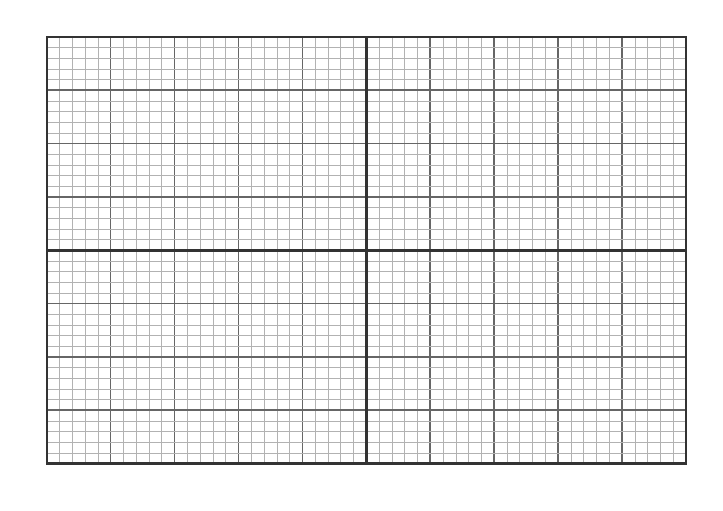
\begin{tikzpicture}
    \begin{axis}[
        width=0.8\textwidth,
        height=7cm,
        grid=both,
        major grid style={line width=.6pt,draw=black!60},
        minor grid style={line width=.2pt,draw=black!30},
        xmin=0, xmax=10,
        ymin=-4, ymax=4,
        xtick={0,1,2,3,4,5,6,7,8,9,10},
        ytick={-4,-3,-2,-1,0,1,2,3,4},
        minor x tick num=4,
        minor y tick num=4,
        xticklabels={},
        yticklabels={},
        tick style={draw=none},
        axis line style={draw=black!80, thick},
    ]
        % Ejes centrales más marcados
        \draw[line width=1pt, black!80] (axis cs:0,0) -- (axis cs:10,0);
        \draw[line width=1pt, black!80] (axis cs:5,-4) -- (axis cs:5,4);
    \end{axis}
\end{tikzpicture}

    \end{figure}

    \begin{figure}[H]
        \centering
        \textbf{ED (Franco Palombo):} Senoidal, \qty{12500}{Hz}, \qty{12.5}{Vpp}, offset: \qty{-10}{V}.
        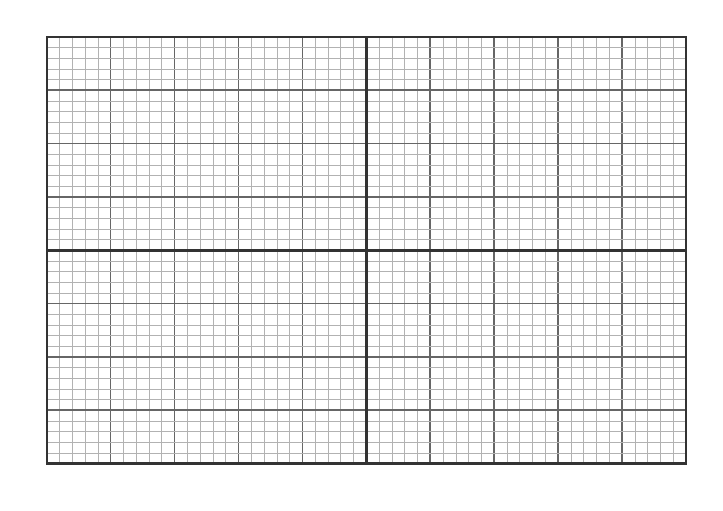
\begin{tikzpicture}
    \begin{axis}[
        width=0.8\textwidth,
        height=7cm,
        grid=both,
        major grid style={line width=.6pt,draw=black!60},
        minor grid style={line width=.2pt,draw=black!30},
        xmin=0, xmax=10,
        ymin=-4, ymax=4,
        xtick={0,1,2,3,4,5,6,7,8,9,10},
        ytick={-4,-3,-2,-1,0,1,2,3,4},
        minor x tick num=4,
        minor y tick num=4,
        xticklabels={},
        yticklabels={},
        tick style={draw=none},
        axis line style={draw=black!80, thick},
    ]
        % Ejes centrales más marcados
        \draw[line width=1pt, black!80] (axis cs:0,0) -- (axis cs:10,0);
        \draw[line width=1pt, black!80] (axis cs:5,-4) -- (axis cs:5,4);
    \end{axis}
\end{tikzpicture}

    \end{figure}
